\chapter{Krav}
Til projektet er der opstillet to krav, som er formuleret i projektoplægget. Det er et krav at disse funktioner implementeres i produktet. Kravene lyder på at der skal udvikles et system, som kan tilsluttes et væskefyldt kateter, samt vise en blodtrykskurve på en computerskærm. Mere detaljeret vil det sige, at systemet skal indeholde to elementer. Først et elektronisk kredsløb, som forstærker signalet fra tryktransduceren og filtrerer det med et indbygget analogt filter. Derefter et program til at vise blodtrykket, som funktion af tiden.

Yderligere skal dette program opfylde kravene:
\begin{itemize}
\item Programmeres i C\#
\item Kunne kalibrere blodtrykssignalet og foretage en nulpunktsjustering
\item Vise blodtrykket kontinuert
\item Kunne lagre de målte data i en tekstfil eller en database
\item Kunne filtrere blodtrykket via et digitalt filter, denne funkton skal kunne slås til og fra
\end{itemize}

På baggrund af disse krav er der opstillet fem Use Cases, der tager højde for disse krav, samt beskriver aktørens interaktion med systemet. Disse Use Cases benyttes som kravspecifikation, der har til formål at specificere, hvilke krav der stilles til projektet. Udover ovennævnte krav vil der også blive arbejdet hen imod at systemet skal afbillede puls, det systoliske blodtryk og det diastoliske blodtryk med tal. \\
Kravene opstilles ud fra kundens ønsker samt leverandørens mulighed for realisering. Systemet består af en computer med programkode, en NI-DAQmx, en transducer og hardware VEVO Board med et filter og en forstærker. Den fulde beskrivelse af hver enkelt Use Cases (fully dressed Use Cases) findes i dokumentationen. 

\begin{figure}[htb]
	\centering
	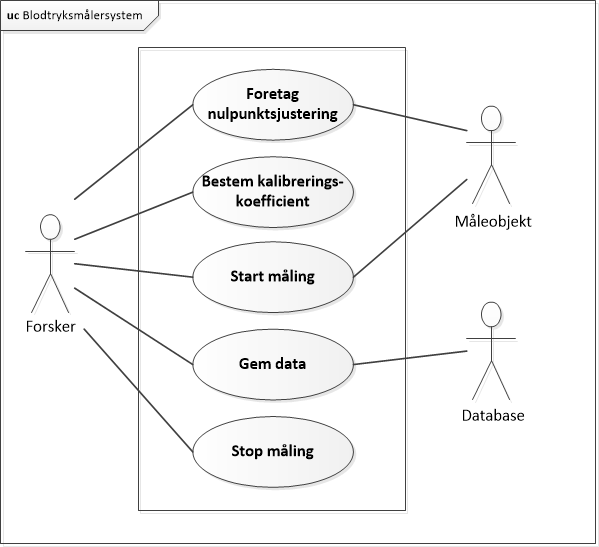
\includegraphics[width=0.6\textwidth]{Figurer/UseCasediagram}
	\caption{Use Case diagram}
	%\label{fig:Use Case diagrammet for blodtrykssystemet}
\end{figure}

\subsubsection{Aktørbeskrivelse}
Use Case diagrammet viser de tre aktører: Forsker, Database og Transducer. Herunder er der en detaljeret beskrivelse af hver aktør.

\textbf{Forsker} er en primær aktør. Det er denne aktør, som foretager blodtryksmålingen, kalibrer og fortager nulpunktsjustering. Målingerne for blodtrykssignalet vises på displayet, som forskeren har tilgang til. 

\textbf{Transducer} er en sekundær aktør. Transduceren har til formål at modtage blodtrykssignalet fra måleobjektet, som kan bestå af In Vitro, patient eller anden, som kan skabe et blodtrykssignal. 

\textbf{Database} er en sekundær aktør. Denne aktør er en database, hvori blodtrykssignalets rådata gemmes. Ligeledes gemmes det indtastede forsøgsnavn og det autogenerede Id.

\subsubsection{Use Case beskrivelse}
Use Case diagrammet viser ligeledes de fem Use Cases, der er for systemet: Foretag nulpunktsjustering, Bestem kalibreringskoefficient, Start Måling, Gem data, Stop måling. Disse Use Cases beskriver interaktionen mellem aktørerne og systemet. Herunder er der en kort beskrivelse formålet med hver Use Case.

\textbf{UC1: Foretag nulpunktsjustering}
Når systemet startes op vil det første der møder forskeren være en GUI, hvorfra nulpunktsjustering kan foretages. Det forudsættes at forskeren har åbnet for transduceren, så den modtager atmosfærisk tryk inden at forskeren trykker på foretag. Systemet indhenter så en nulpunktsjusteringsværdi, denne værdi gemmes i softwaren og alt indhentet signal herefter vil dermed være indstillet til en offset på nul. Herefter går systemet videre til næste Use Case

\textbf{UC2: Bestem kalibreringskoefficient}
Kalibreringen foregår uafhængig af om systemet kører. Forsker tilslutter hardware til væskesøjle ved 50 mmHg. Så aflæses output spænding fra hardwaren. Kalibreringskoefficienten kan så bestemmes ved en simpel beregning ud fra tryk og output spænding. Denne værdi indtastet så i fil, hvorfra softwaren kan tilgå koefficienten og derefter benytte den som omsætningskoefficient mellem volt og mmHg. Dermed er en kalibrering udført.   

\textbf{UC3: Start måling}
Det kræves at måleobjekt, hvorpå blodtrykssignal ønskes fra, er tilsluttet. Derfor tilslutter forskeren transduceren til måleobjektet. Derpå kan målingen startes ved, at forskeren trykker på knappen START MÅLING. Herefter indhenter systemet blodtrykssignalet, som bliver udskrevet på display. Værdier for puls, systolisk- og diastolisk blodtryk udskrives på display. 

\textbf{UC4: Gem data}
Det er muligt for forskeren at gemme det indhentede blodtrykssignals rådata, indenfor en periode, valgt af forskeren. Dette gøres ved, at forskeren trykker på knappen START GEM. Systemet vil herefter begynde at sende rådata ind i databasen, hvor dataene gemmes. Dette vil systemet blive ved med at udføre indtil forskeren trykker på knappen STOP GEM. Ved tryk på STOP GEM vises filnavn på display. 

\textbf{UC5: Stop måling}
Det er muligt for forskeren at stoppe visning af blodtrykssignalet. Dette gøres ved, at forskeren trykker på knappen STOP MÅLING. Systemet vil herefter lukke forbindelsen til indhentning af data og grafen i chart vil fastholdes. 

\subsubsection{Ikke-funktionelle krav beskrivelse}
Ikke-funktionelle krav er struktureret efter (F)URPS+, hvor krav til systemets funktionalitet, brugervenlighed, pålidelighed, præsentation samt vedligehold er beskrevet. Disse krav er primært software-krav. Der opstilles bl.a. et krav om en maksimal tid, der må gå fra, at der er trykket på en knap, til at systemet reagerer. Når der er trykket på en knap, skal systemet foretage den ønskede proces, hvilket eksempelvis er, at ved tryk på GEM-knappen, at sende det ufiltrerede blodtrykssignal til databasen, hvor signaldata bliver gemt. Ligeledes er opbygning af display også en del af de ikke-funktionelle krav.